%%%%%%%%%%%%%%%%%%%%%%%%%%%%
% Master's Thesis          %	    										
% Fabian Burth, 2022-08-01 %
%%%%%%%%%%%%%%%%%%%%%%%%%%%%

\npchapter{Result}
After the technical and architectural design decisions are discussed in detail, this chapter finally presents the results, thus, the actual functionality of the \emph{Security and Compliance Data Lake} in practice. Furthermore, the design decisions, the implementation and thereby, the actual value of this research based practical contribution to increase the trust and transparency placed in our digital infrastructure, are evaluated. To conclude this work, the research question is revisited, summarizing the greatest challenges throughout the application design and development. 

\section{Presentation} \label{sec:Presentation}
This presentation section briefly introduces the infrastructure, the data model configuration and the data set of the application instance used to demonstrate the functionality, before showing queries answering interesting questions about software composition through the GraphQL API. After all, the \emph{Security and Compliance Data Lake} is a backend application providing its functionality through a standard interface, GraphQL, and returning its results in a machine readable format, JSON, limiting the possibilities for impressive visual showcasing.   

\subsection{Application Infrastructure}
Originally, the application was developed and tested in \emph{Windows Subsystem for Linux 2 (WSL2)} on a windows machine. Thus, the database as well as the application was running there.\par
After the first PoC of the application was finished, SAP Gardener was used to set up a kubernetes cluster to host presentable versions of the application. Therefore, a simple development pipeline was configured with \emph{GitHub Actions} to automatically containerize the application and push the respective image into a \emph{DockerHub} repository. Furthermore, \emph{kubernetes deployment files} were created, to deploy the application itself, as well as other kubernetes resources such as an \emph{ingress} to expose the API. To deploy the Neo4j database, the corresponding \emph{helm chart} provided by Neo4j was leveraged. Additionally, in order to being able to perform all operations to deploy and undeploy all kubernetes resources at once, a small bash script was set up.\par
In this kubernetes cluster, all resources are deployed on a single \emph{worker node}, hence, a single machine, with 4 CPUs and 16Gi of RAM. Furthermore, the cluster has 50Gi of persistent memory.

\subsection{Application Configuration \& Data}
The \emph{data model} configured through the \emph{Types API} for this application's instance which is used for presentation purposes corresponds to SAP Gardeners \emph{Open Component Model} and the usage of \emph{Black Duck Binary Analysis} as scanning tool and sole \emph{data source}.\par
Thus, the \emph{data} created through the \emph{Consumption API} is provided by a \emph{Component Descriptor Repository} and \emph{Black Duck Binary Analysis}. The presentation application instance contains 22.204 \emph{nodes} and 97.335 \emph{relationships} between those \emph{nodes}. Figure \ref{fig:Neo4jGraph} shows a visual representation of a part of the graph\footnote{The Neo4j web interface becomes unresponsive and aborts the request if the amount of nodes and relationships to be rendered becomes to high. Therefore, it is not possible to show a visual representation of the entire graph here.} rendered by Neo4j to showcase the database's functionality and to give a better feeling for the data.\par

\begin{figure}[H]
	\centering
	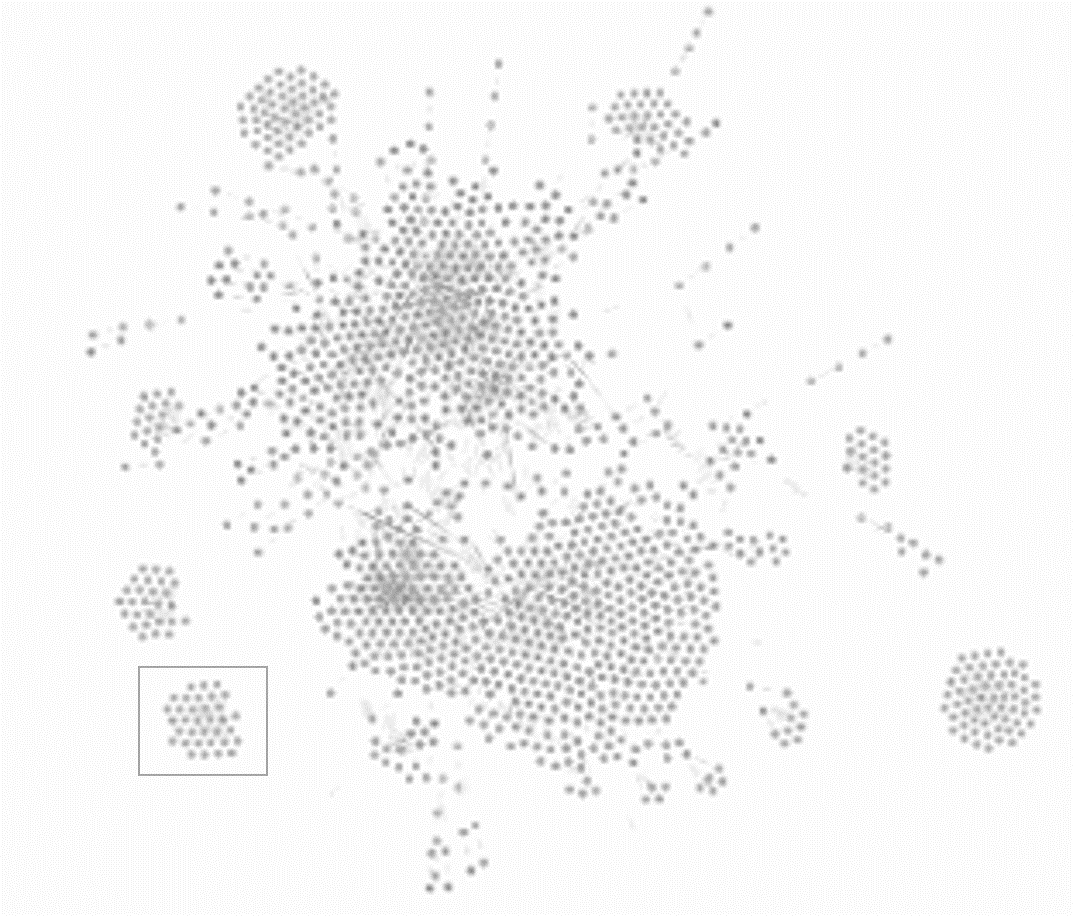
\includegraphics[scale=1.0]{neo4j_graph}
	\caption[Neo4j Graph]{Neo4j Graph Representation \source{Own Representation}}
	\label{fig:Neo4jGraph}
\end{figure}

Although the lines connecting different nodes and thereby representing the relationship are barely visible and often not explicitly rendered, Neo4j visualizes nodes that are highly interrelated close together leading to these visible clusters. The main clusters in the middle revolve around \emph{Component Versions} and contain all kinds of nodes. The larger clusters on the side are \emph{Package Versions} with an exceptionally high number of \emph{Vulnerabilities}. For example, the highlighted cluster on the bottom left revolves around a version of \emph{HashiCorp's Vault}, a software package for managing secrets and protecting sensitive data \cite{vault}.\\

Although this is difficult to arrange clearly, to give a even better understanding of how the data model manifests itself in form of nodes and relationships, figure \ref{fig:Neo4jComponentTree} zooms on a specific component.

\begin{figure}[H]
	\centering
	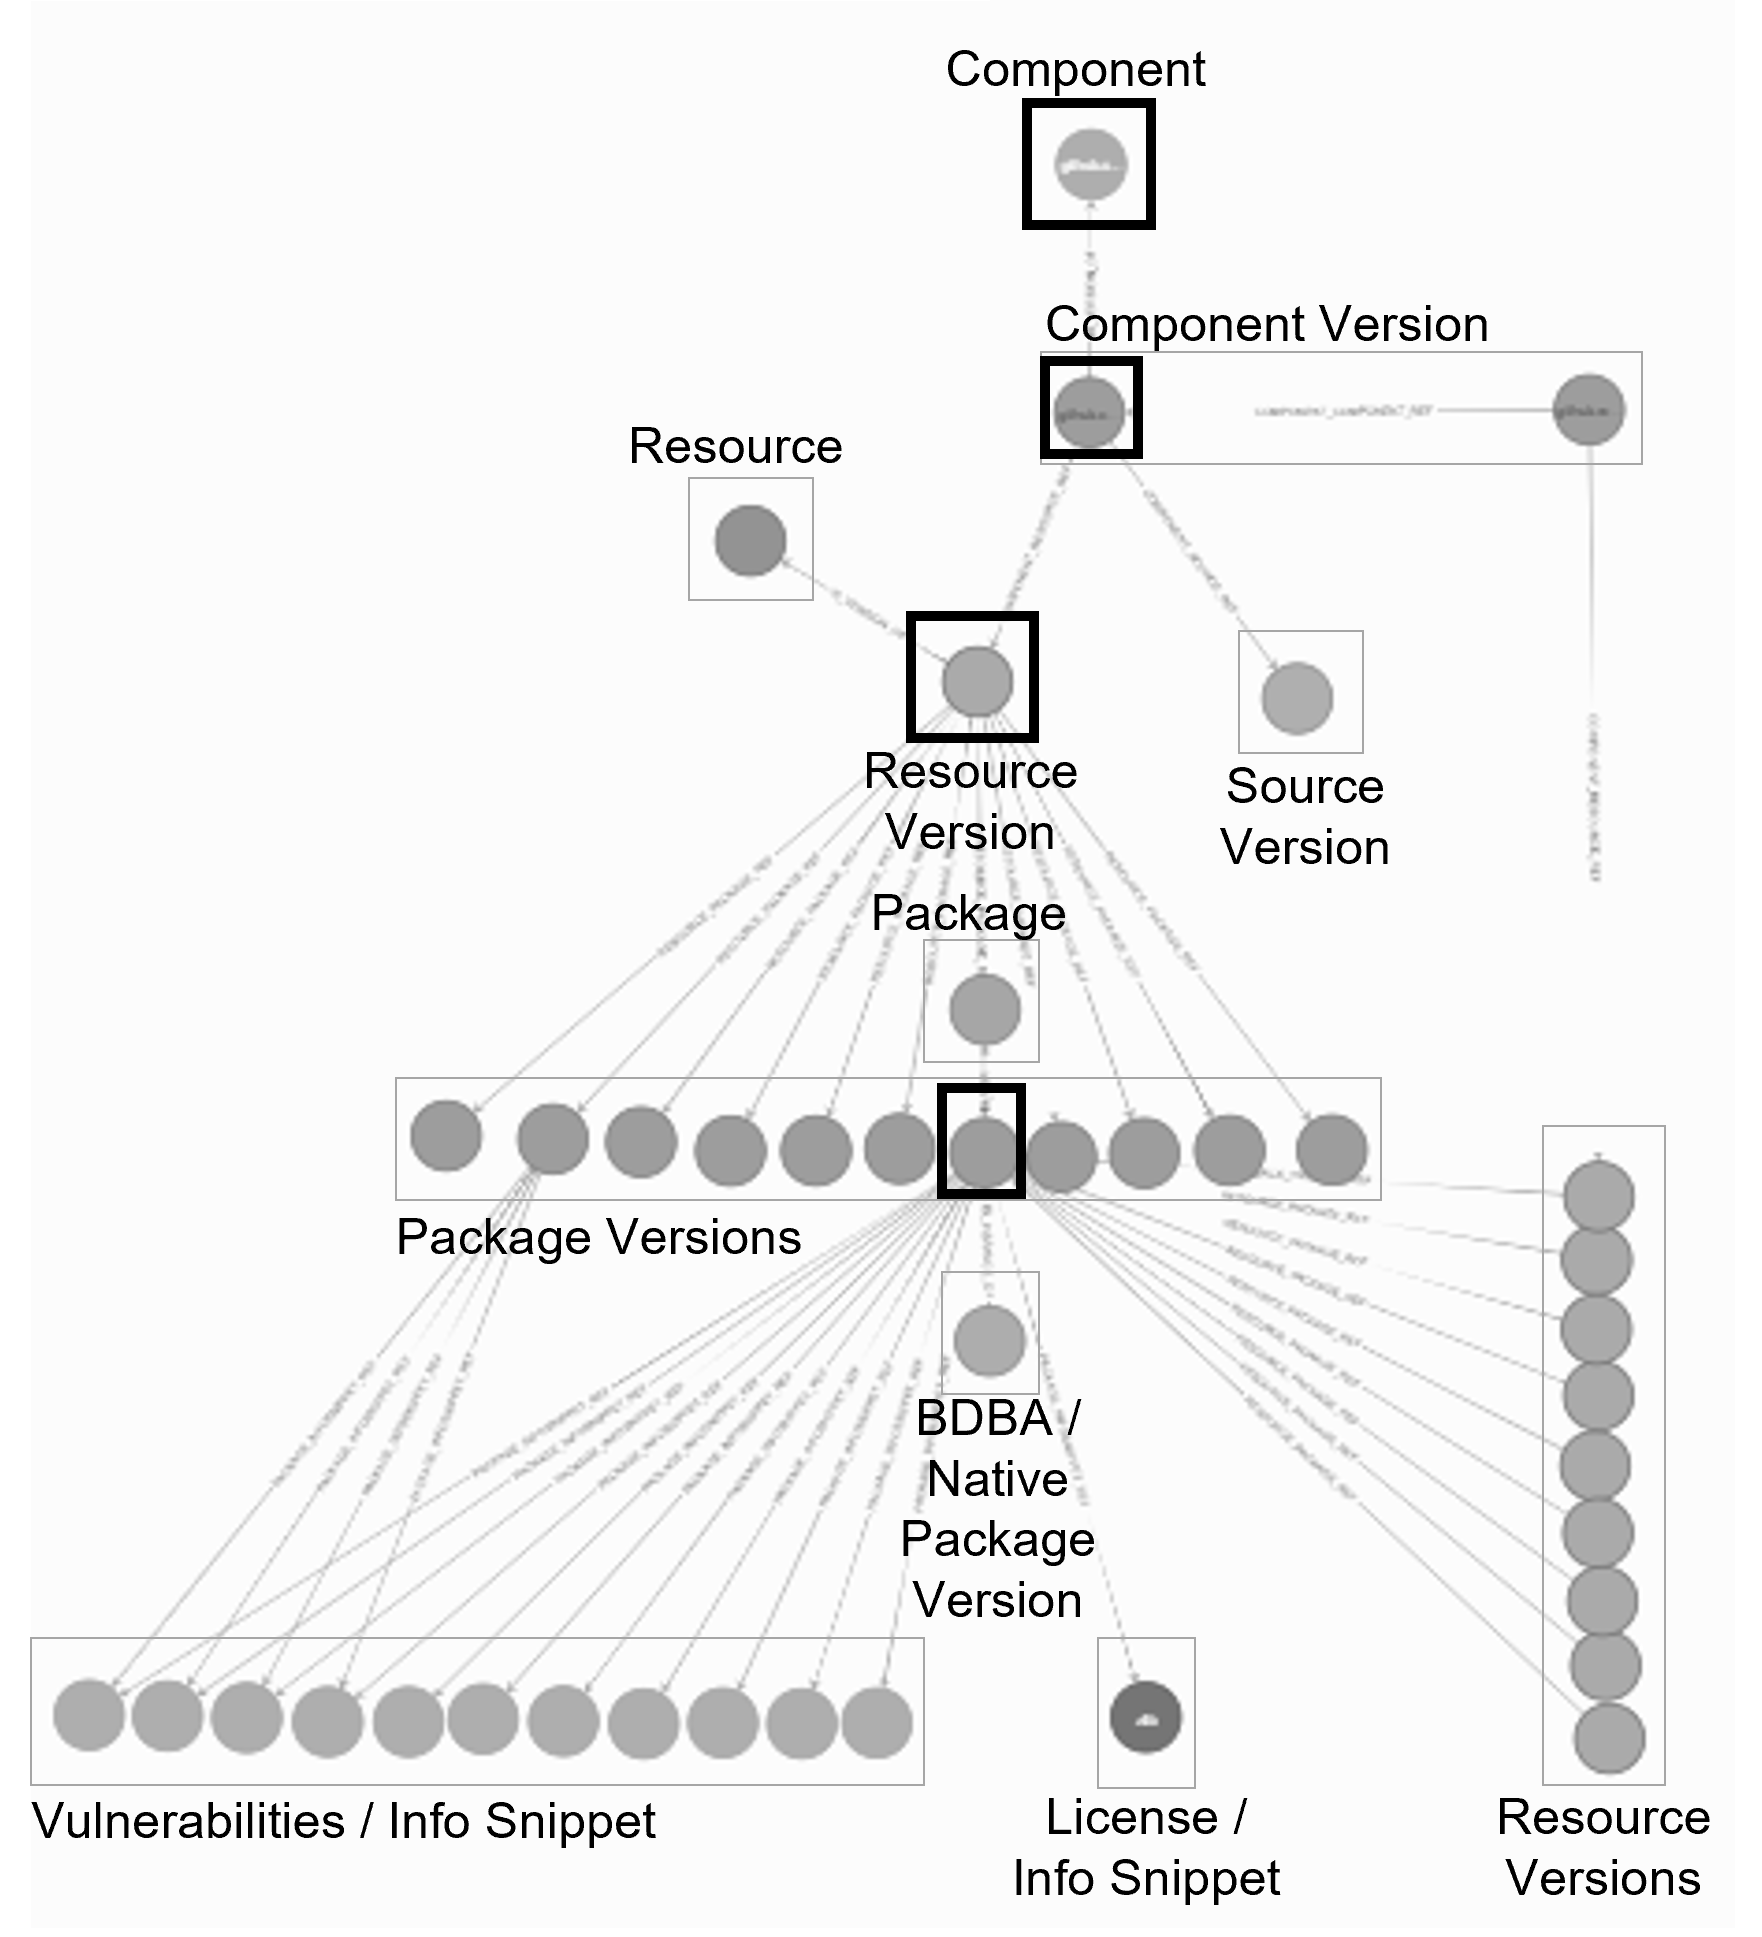
\includegraphics[scale=0.70]{neo4j_graph_zoomed}
	\caption[Neo4j Component Tree]{Neo4j Component Tree Representation \source{Own Representation}}
	\label{fig:Neo4jComponentTree}
\end{figure}

The figure shows a part of the tree formed by the relationships of the \emph{Component} at the top.\footnote{This visualization rendered by Neo4j also shows the names of relationships along the lines and the names of some nodes within the circle. These are not intended to be readable in this figure. They are not important for the explanations and there is no way to zoom in close enough to keep them readable while still showing the whole tree.} To be more precise, the nodes that are highlighted by a thicker black border are the ones that are unfolded. Thus, for these nodes all related nodes are visualized.\par
The \emph{Component} at the top has only one relationship to a \emph{Component Version}. Thus, there is only one version of this \emph{Component} stored in the database. As the highlighted \emph{Component Version} straight under the \emph{Component} is unfolded, the figure shows that it references one other \emph{Component Version}. Moreover, it also references a \emph{Resource Version} and a \emph{Source Version}. Since the \emph{Source Version} is not unfolded, its related nodes are not shown. If it was unfolded, it would most likely open up a subtree similar to the one of the highlighted and therefore unfolded \emph{Resource Version}. The same is true for the \emph{Resource}. If it was unfolded, it would possibly show several more \emph{Resource Versions}. Besides the \emph{Resource}, the unfolded \emph{Resource Version} is especially related to several \emph{Package Versions}. The unfolded \emph{Package Version} is related to its other two aggregation levels, \emph{Package}, shown directly above it and below \emph{Resource Version}, and \emph{BDBA}, or rather, \emph{Native Package Version}. The relationships to the \emph{Resource Versions} on the right show that this particular \emph{Package Version} occurs in several more \emph{Resource Versions}. The topmost \emph{Resource Version} is even referenced by the \emph{Component Version} which is referenced by the unfolded \emph{Component Version}. Thus, there are two different paths through which this particular \emph{Package Version} is contained in the \emph{Component}. Furthermore, the \emph{Package Version} is related to, or rather has, a number of \emph{Vulnerabilities} and a \emph{License} which are both \emph{Info Snippets}. The \emph{Vulnerabilities} on the left even occur within another \emph{Package Version}.\par 
So, although this has been theoretically discussed before, this conveniently visualizes the paths that have to be traversed to answer questions related to software composition.


\subsection{Demonstration}
The \emph{data model configuration} is not really interesting, as it is just sending several schemas to the respective endpoint. There is not much more to show than what was already presented in section \ref{sec:Types API & Services} "Types API \& Services. Moreover, these schemas are SAP Gardener OCM specific and are even provisional for the PoC. For the productive use of the application, these will have to be adjusted in close cooperation with the corresponding stake holders within the SAP Gardener Team.\par
The \emph{data upload} is handled by an \emph{Adapter} written in \emph{Python}. This \emph{Adapter} is tailored for the PoC use case. Therefore, the upload may be triggered manually by specifying a specific \emph{Component Version}. Consequently, all the \emph{References} to other \emph{Component Versions}, to \emph{Resource Versions} and  \emph{Source Versions} are resolved recursively and uploaded to the \emph{Security and Compliance Data Lake} in the correct order, so that the application does not attempt to create a relationship to an entity that may not exist yet. Furthermore, the \emph{Adapter} retrieves the scan results for respective \emph{Resource Versions} from the BDBA API and uploads as well. The actual scans are triggered independently. This way, the results may be uploaded without performing a scan every time which is especially useful during development.\par
Finally, the \emph{data analysis} may be performed through the GraphQL API. To demonstrate the functionalities and capabilities of the \emph{Security and Compliance Data Lake}, the following paragraphs show how it may be used to answer questions about software composition. The application is currently not connected to a front end. Therefore, provisionally, the only way to retrieve specific data is to actually type the respective request body. To make this more comfortable, the \emph{Security and Compliance Data Lake} also hosts \emph{GraphiQL}, a Web IDE for GraphQL, offering syntax highlighting, auto-completion and automatic documentation \cite{graphiql}. This Web IDE is also used for running the following queries.\\

Throughout the thesis, the two most common questions were, \emph{"Which Vulnerabilities are contained in a specific Component Version?"} and the reciprocal \emph{"Which Component Version contains a specific Vulnerability?}.\par
So, to address the first question, a \emph{Component Version} has to be picked. For this presentation, the \emph{github.com/gardener/dashboard} version \emph{1.64.0} is used. This \emph{Component} is somewhat tangible as it represents actual releases of the \emph{SAP Gardener Dashboard}, a web application to monitor OCM components, which incidentally will prospectively also leverage the \emph{Security and Compliance Data Lake} to extend its functionality.

\begin{figure}[H]
	\centering
	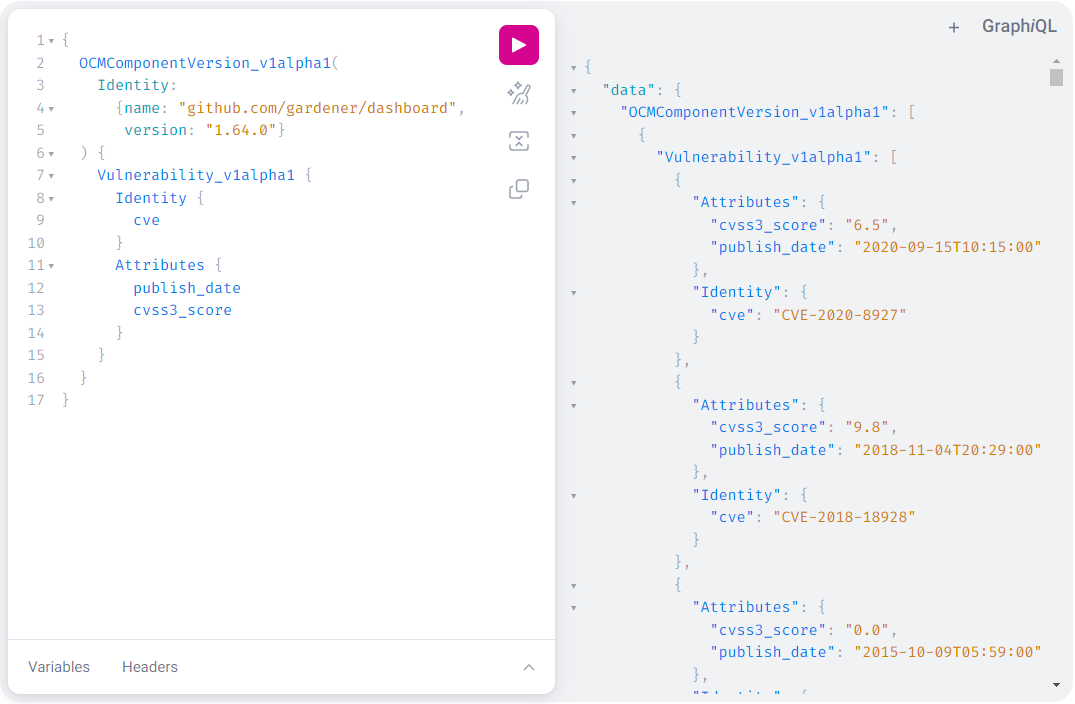
\includegraphics[scale=0.52]{graphiql_component_vulns_query}
	\caption[Vulnerabilities in Component]{Vulnerabilities in Component \source{Own Representation}}
	\label{fig:VulnsInComp}
\end{figure}

The screenshot from the GraphiQL Web IDE shows the GraphQL query on the left and the corresponding response on the right. The query specifies to return the \emph{Identity} property \emph{cve} and the \emph{Attribute} properties \emph{publish date} and \emph{cvss3\_score} for each \emph{Vulnerability} in the \emph{Component Version}. The right side shows that the query returns a JSON document containing an array of \emph{Vulnerabilities}. Thereby, the scrollbar indicates the array contains several more \emph{Vulnerabilities} than visible in the screenshot. As briefly mentioned in section \ref{sec:Meta Data Model} "Meta Data Model", the entity type schemas themselve may be versioned. Since schema names in GraphQL have to be unique, a suffix, in above figure \emph{v1alpha1} accounts for this schema versioning.\par 
To demonstrate how to answer the reciprocal query, the upper most \emph{Vulnerability} with the \emph{cve} of \emph{CVE-2020-8927} in above figure is used. 

\begin{figure}[H]
	\centering
	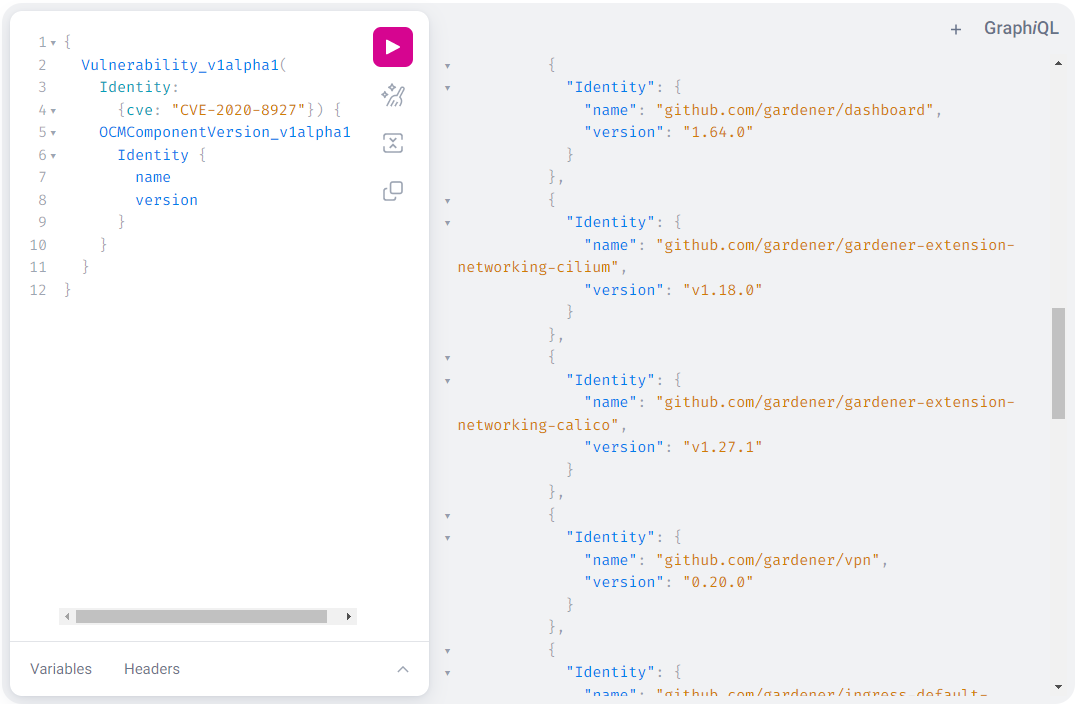
\includegraphics[scale=0.52]{graphiql_vulns_comp_query}
	\caption[Components with Vulnerability]{Components with Vulnerability \source{Own Representation}}
	\label{fig:CompsWithVuln}
\end{figure}

The result in figure \ref{fig:CompsWithVuln} is scrolled down a bit, as indicated by the scrollbar, to show that the array of \emph{Component Versions} naturally also contains the \emph{Component Version} where the \emph{Vulnerability} was found in in the example before. The poupular question \emph{"Which Deployments contain the Log4j vulnerability} could be answered correspondingly.\par
To further stress the capabilities of the GraphQL, the following query shows how to query all \emph{Package Versions} contained in the \emph{github.com/gardener/dashboard} \emph{Component Version} and return the respective \emph{Licenses} at the same time.

\begin{figure}[H]
	\centering
	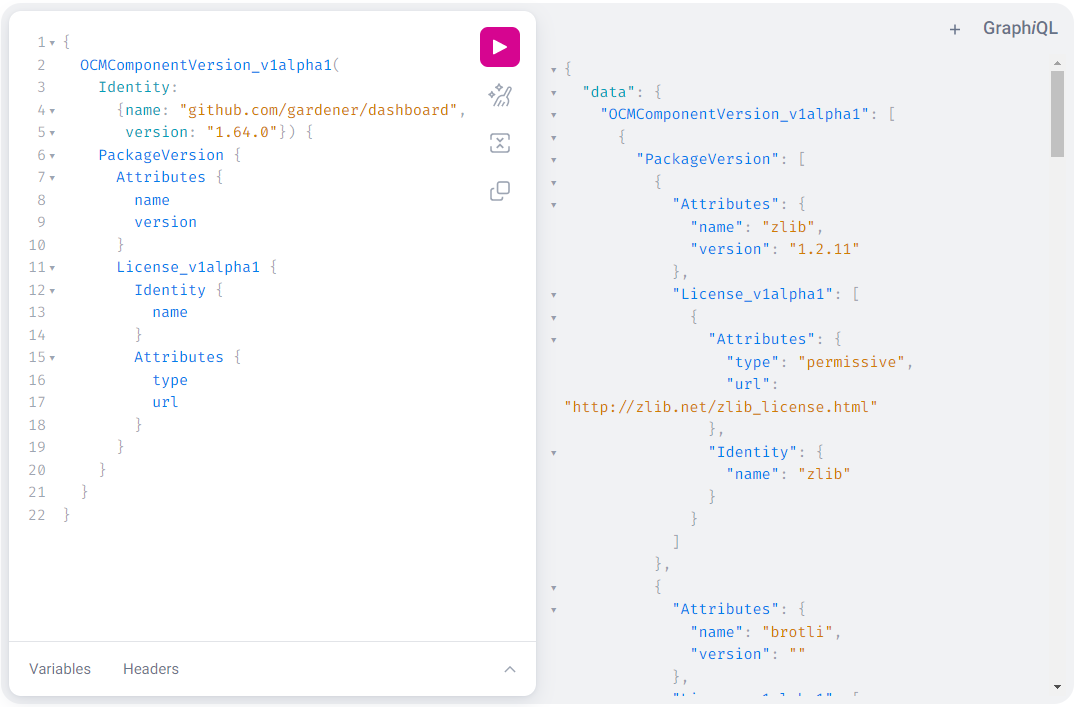
\includegraphics[scale=0.52]{graphiql_comps_pkg_license}
	\caption[Packages in Component]{Packages in Component \source{Own Representation}}
	\label{fig:CompWithPkgs}
\end{figure}

Figure \ref{fig:CompWithPkgs} shows that the result is a JSON document containing an array of \emph{Package Version} and again, nested in each \emph{Package Version}, an array of \emph{Licenses}. Thus, the queries may even be nested.\\

There is a lot more functionality that could be showcased. But as the above examples are sufficient to convey a basic understanding of the functionality and each further example takes up a lot of space, the following sections transition to an evaluation. 

\section{Evaluation}
The evaluation starts with a review of the application's requirement fulfillment. Some of this information is already discussed alongside the limitations and problems of the application architecture in section \ref{sec:Limitations and Problems}, which focuses on restrictions imposed by the architecture itself and therefore requiring considerable adjustments to resolve. In contrary, the following section provides a more holistic view, summing up how each requirement is fulfilled by the application or what has to be done in order to satisfy a currently unfulfilled requirement. Moreover, challenges, efforts and difficulties in the development process that may not have been explicitly visible throughout the thesis are briefly addressed and the research question is revisited.

\subsection{Requirements}
To provide a closing evaluation of the PoC implementation of the \emph{Security and Compliance Data Lake} developed during this scientific work, the currently available functionality is compared to the requirements specified in section \ref{sec:Requirements}.\par
\emph{Requirement R.1} specifies that the application shall be able to consume and store metadata from multiple different data sources. This was a crucial aspect during data model and application design as also stressed in the corresponding chapters. The data model introduced \emph{classes of entity types} to express this extensibility and the application architecture exposes the \emph{Types API} to dynamically create and configure the actual data model tailored to the respective use case. As the application thereby provides the possibility to not just configure different data sources for package information such as BDBA and Mend, but to even configure the \emph{component model} and theoretically supports the option to use multiple \emph{component models} in parallel, requirement R.1 is exceeded.\par
\emph{Requirement R.2} is to store the metadata from different data sources without aggregation. The data model splits the package type into three aggregation levels, \emph{Package}, \emph{Package Version} and \emph{Native Package Version}. On the \emph{Native Package Version} aggregation level, the metadata for a package may be stored as provided by the respective data source without the necessity to merge, or rather aggregate, the data. Thus, requirement R.2 is fulfilled.\par
The \emph{Package Version} aggregation level is intended to store the aggregated data. As described in the meta data model, the \emph{Native Package Version} schema therefore has to specify the attributes specific to the data source, the \emph{native attributes} and the attributes that shall be aggregated, the \emph{attributes}. Although the current implementation creates this aggregate level implicitly, the merging has to be done manually. The API currently does not expose an operation to do this. Therefore, while the application architecture and design are prepared to fulfill this functionality, it currently is not available and is yet to be added. So requirement R.3 is not completely fulfilled. As the SAP Gardener team for whom the application was primarily developed, currently only actively uses a single data source for this kind of information, BDBA, the actual implementation of the requirement had a lower priority for the PoC.\par
\emph{Requirement R.4}, providing an aggregation level to group sources and resources, is implemented through the component entity types. Thereby, the application bridges the gap between artifact metadata and deployment information.\par
\emph{Requirement R.5} is probably the most visible and is based on several of the previously mentioned requirements. As discussed in section \ref{sec:Query API & Services} and also shown in the previous presentations, the GraphQL API enables users to easily query the metadata on different levels of aggregation. Thus, questions such as which vulnerabilities are contained in a specific resource or in a specific deployment may be answered effortlessly. The underlying complex graph traversals necessary to query this information are thereby completely transparent to the user.\par
As already discussed in section \ref{sec:Limitations and Problems} "Limitations and Problems" of the application's architecture, \emph{Requirement R.6} currently is not fulfilled by the PoC. Either, an extension of the \emph{Types API} and respective services or a static extension of the schemas will have to be added.\par
\emph{Requirements R.7}, to provide aggregation and filter functions, and \emph{Requirement R.8}, to enable querying the metadata in common SBOM formats, are not implemented either. But based on the application's architecture, these functionalities may easily be added.\\

Regarding \emph{non-functional requirements}, no specific boundaries were defined. Still, it is mentioned several times that performance, especially of read operations, is relevant. Neither the amount of data in the presentation application instance, nor the compute resources of the cluster correspond exactly to the conditions of a productive application instance.\par
Anyway, as a point of orientation, the queries performed in section \ref{sec:Presentation} usually return in approximately 1-5 seconds, also depending on the internet connection and the amount of data requested.\par 
Theoretically, especially the performance of "top-down queries", thus, queries answering questions like which \emph{Vulnerabilities} are contained in a \emph{Component Versions}, should stay relatively constant even with far more nodes in the graph over all. "Top-down" as \emph{Component Versions} build up a tree that is self-contained and aside of some discovered vulnerabilities (and possibly other \emph{Info Snippets}) usually stays relatively constant the same over time. Thus, corresponding to the explanations in section \ref{sec:GraphDB Theoretical Foundation}, the look up of the initial node is the only part of the query which may decrease significantly in performance. An important side note at this point, this is only true for "top down" queries starting on \emph{Component Version} level and below, as the number of \emph{Component Versions}, and thus, the number of entire trees under a \emph{Component} will naturally grow significantly over time.\par
Generally, a similar concept applies to most of the "bottom up queries". So, answering questions like which \emph{Component Versions} contain a specific \emph{Package Version} naturally spans several of the \emph{Component Version} trees. But as new \emph{Component Versions} will generally also switch to newer \emph{Package Versions}, this growth is also limited in most cases.\par
Thus, theoretically, the query performance should scale quite good, as most of them are likely limited to self-contained subgraphs.\\

To summarize this, the current PoC of the \emph{Security and Compliance Data Lake} implements almost all of the \emph{priority 1} requirements R.1 - R.5. Thereby, the application is already able to perform the most relevant queries and analysis about software composition and answer important questions such as \emph{"which deployments contain the Log4j vulnerability?"} within seconds. As shown by the system design section, the decisions which lead the application design and the application's architecture are based on thorough research. Thus, the application definitely poses a scientific and practical contribution to increase the transparency of our digital infrastructure.\par
Furthermore, the reasons for not fulfilling the other requirements are not actual hard limitations of the application's architecture, but merely the lack of time. So, the currently missing functionality may be added in future.

\subsection{Research Question and Retrospective}
As common in software development, or rather in science in general, the complexity of a problem only really unfolds, once one actually starts trying to solve it. Correspondingly, the complexity to design and develop a sustainable solution for such a software metadata store and provide a sustainable solution became much bigger than originally anticipated. This section sums up the thesis, highlighting the greatest challenges and concluding with a retrospective onto implementations and decisions.\\

First of all, the \emph{requirement elicitation} was an important part of this work. Due to the versatile ecosystem concerning software supply chain security and software metadata, this tasks proved challenging. Therefore, \emph{chapters 2 and 3} not only serve as foundation for the reader, but serve as valuable preparation for the entire work. \emph{Chapter 2} provides an overview and basic understanding of the subject area and its existing standards and technologies. Thereon, \emph{chapter 3} introduces the current state of the art approach, pointing out its limitations, such as the coupling of CI and CD,the distribution of the software metadata over the software development life cycle and the resulting informational gap between artifacts and deployments.\\
\emph{Chapter 4} is focused on SAP Gardeners Open Component Model. The Open Component Model allows for decoupling CI from CD and provides a convenient and practice proved starting point for the design of a generic data model connecting artifact metadata with deployment metadata. Furthermore, it serves as a reference of how to integrate the Open Component Model and the \emph{Security and Compliance Data Lake} into a modern development and deployment landscape, thereby stressing their practical applicability. As the Open Component Model and its tooling is itself relatively new, the documentation still lacks depth, explanations and extensive examples. Therefore, collecting the respective information included a lot of interviews and discussions with the responsible developers which were particularly difficult due to the abstract nature and the ambiguous terms of the Open Component Model. Consequently, this supposedly simple task of \emph{familiarizing with and explaining of existing concepts and tools}, turned out to be a real challenge.\\

\emph{Chapter 5} concludes the efforts of the previous chapters, leveraging the preparations to specify requirements and to design an entire software system. Thereby, the greatest challenges were the \emph{inconsistency of identities} and the \emph{volatility, or rather unpredictability, of the data model}.\par
The problem around artifact identities, thus, the ambiguity of artifact references regarding the actual technical artifacts, has been discussed in detail in the context of component models. But even more generally, in order to being able to reliably identify data delivered from different data sources as data about the same entity, this entity needs a \emph{globally unique identifier}. Although there are efforts to establish standards for identifying different entities, such as \emph{PURL} for packages or the \emph{SPDX License Identifier} for licenses, these are rarely used by scanning tools at all or at least not consistently.\par
Considering the unpredictability of the data model, extending the entity relationship model with classes of entity types added some complexity to the explanations but was not particularly difficult itself. But dealing with such a generic data model during system design was. Thus,  providing an architecture which enables enforcing the data model while maintaining the extensibility and flexibility to add new entity types and even configure the properties of entity types dynamically at runtime. Therefore, coming up with the \emph{Meta Data Model}, implementing code on the data source logic layer that \emph{constructs the statements in the database's query language, cypher, based on the concrete data model configured by the user} and developing \emph{APIs that dynamically adjust to this concrete data model}. So, if the user creates a new \emph{Info Snippet Type}, for example \emph{Build Information}, the \emph{Consumption API} subsequently also considers this entity type during \emph{validation}. Simultaneously, the \emph{Query API} automatically adds an option to query entities of type \emph{Build Information} based on their respective properties.\par
Besides, the research to determine the best database technology for the application was time intensive. But, as the decision to use a graph database was questioned by colleagues and peers, the research has been proven to be worthwhile. Most of the skepticism may be traced back to unfamiliarity and has been mostly eliminated by the successful PoC of the \emph{Security and Compliance Data Lake}.\\

Furthermore, 

\section{Related Work}

\section{Outlook}
index creation



